\documentclass[a4paper,12pt]{article}
\usepackage[utf8]{inputenc}
\usepackage{polski}
\usepackage[left=2.5cm,right=2.5cm,top=2.5cm,bottom=2cm]{geometry}
\usepackage{mathtools}
\usepackage{amsmath}
\usepackage{latexsym}

\title{Sprawozdanie P0.2}
\author{Kamil Tasarz, 322492}
\date{październik 2021}

\begin{document}

\maketitle

\section{Wstęp}

Celem tej pracowni jest napisanie przykładowego sprawozdania, zapoznanie się z technicznymi zasadami zaliczania pracowni oraz wysłanie sprawozdania w Portalu Przedmioty.

\section{Działy i poddziały}

\subsection{Poddział 1}

Treść pierwszego poddziału pierwszego rozdziału.

\subsection{Drugi poddział}

COŚ

\section{Tabela zawierająca liczby}

\begin{center}
\begin{tabular}{|c|c|c|c|c|} \hline
\multicolumn{5}{|c|}
{to jest tabela zawierająca liczby} \\ \hline
10 &  1 &  1.0657120621 &  1.06571206217 &  17\\
\hline
20 &  23 &  177 &  3.965172E-0007 &  17\\
\hline
55555555 &  2.23092008061E-0009 &  2.2 &  -9 &  17\\
\hline
1 &  3 &  7 &  2.0 &  17\\
\hline
1 &  3 &  7 &  2.0 &  17\\
\hline
1 &  3 &  7.0 &  2 &  17\\
\hline
1.0 &  3.0 &  7 &  12 &  17\\
\hline
1 &  35 &  575 &  22345678 &  17\\
\hline
\end{tabular}
\end{center}

\newpage

\section{Wykres}

\begin{figure}[ht]
  \begin{center}
  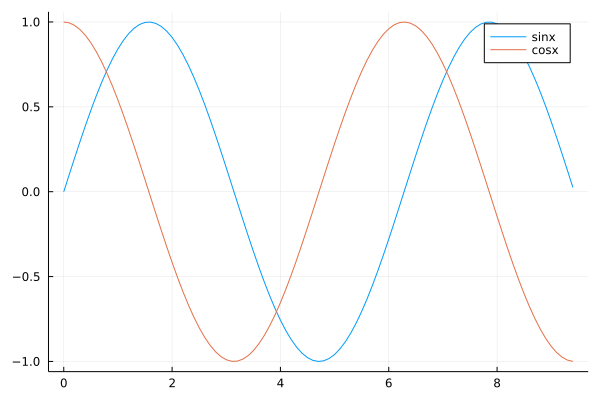
\includegraphics[width=10cm]{wyk.png}
  \end{center}
  \label{fig:rysunek}
\end{figure}

\section{Twierdzenie Taylora (o szeregu)}

Niech f będzie funkcją na przedziale [a, b] o wartościach rzeczywistych (bądź ogólniej, o wartościach w przestrzeni unormowanej Y) różniczkowalną (n + 1)-razy w sposób ciągły (na końcach przedziału zakłada się różniczkowalność z lewej, bądź odpowiednio, z prawej strony). Wówczas dla każdego punktu x z przedziału (a, b) spełniony jest wzór zwany wzorem Taylora:

\begin{align*}
 f(x) & = f(a) + \frac{x-a}{1!}f^{(1)}(a) + \frac{(x-a)^2}{2!}f^{(2)}(a) + \dotsb + \frac{(x-a)^n}{n!}f^{(n)}(a) + R_n(x, a) \\
 &= \sum_{k=0}^n \left( \frac{(x-a)^k}{k!}f^{(k)}(a) \right)+ R_n(x, a),
\end{align*}
gdzie $f^{(k)}(a)$ jest pochodną k-tego rzędu funkcji $f$ obliczoną w punkcie $a$, przy czym $R_{n}(x,a)$ spełnia warunek 
\begin{flalign*}
&\lim_{x\to a}\frac{R_{n}(x,a)}{||x-a||^n} = 0.&
\end{flalign*}
\end{document}
